\newpage
\appendix
\appendixpage
\addappheadtotoc


\chapter{Project management forms}
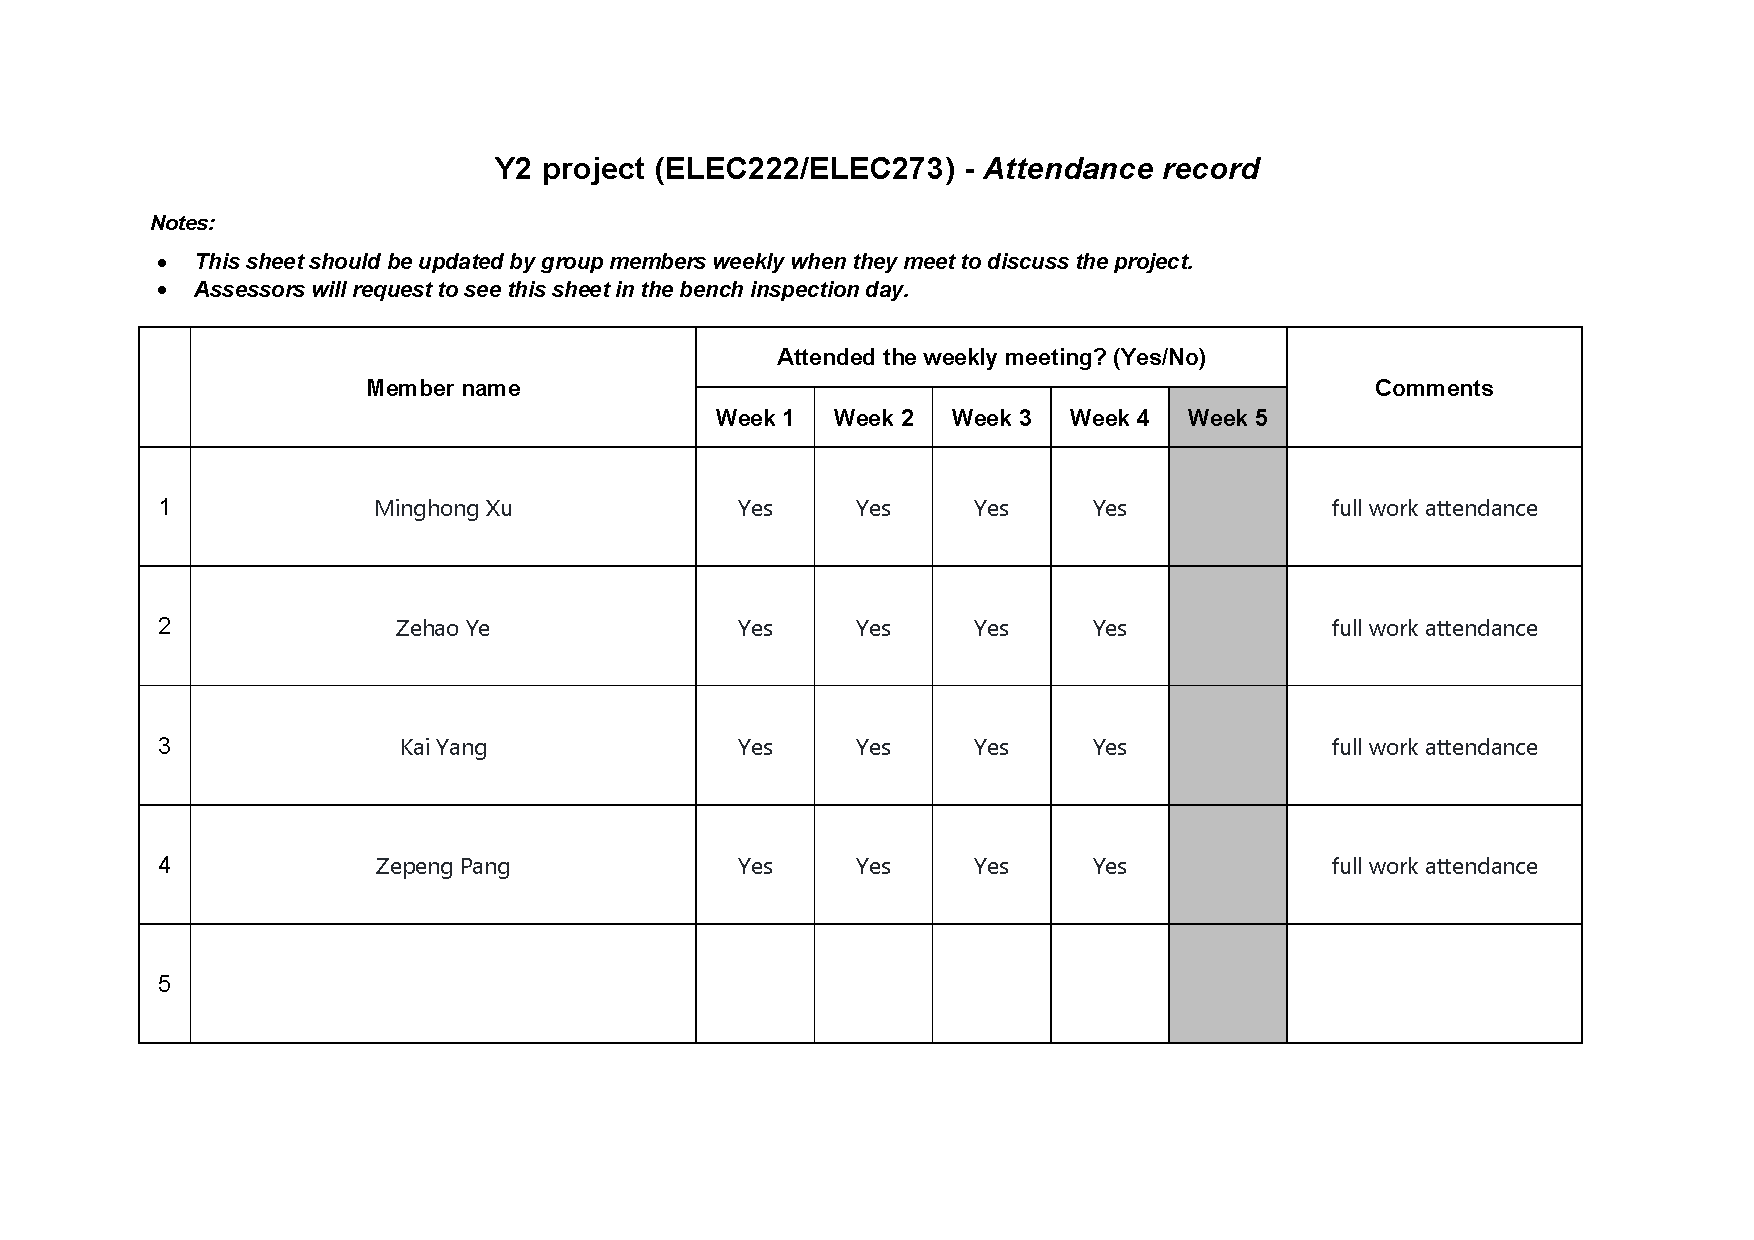
\includepdf[pages=-]{../proj_mgmt_forms/attendance_record.pdf}
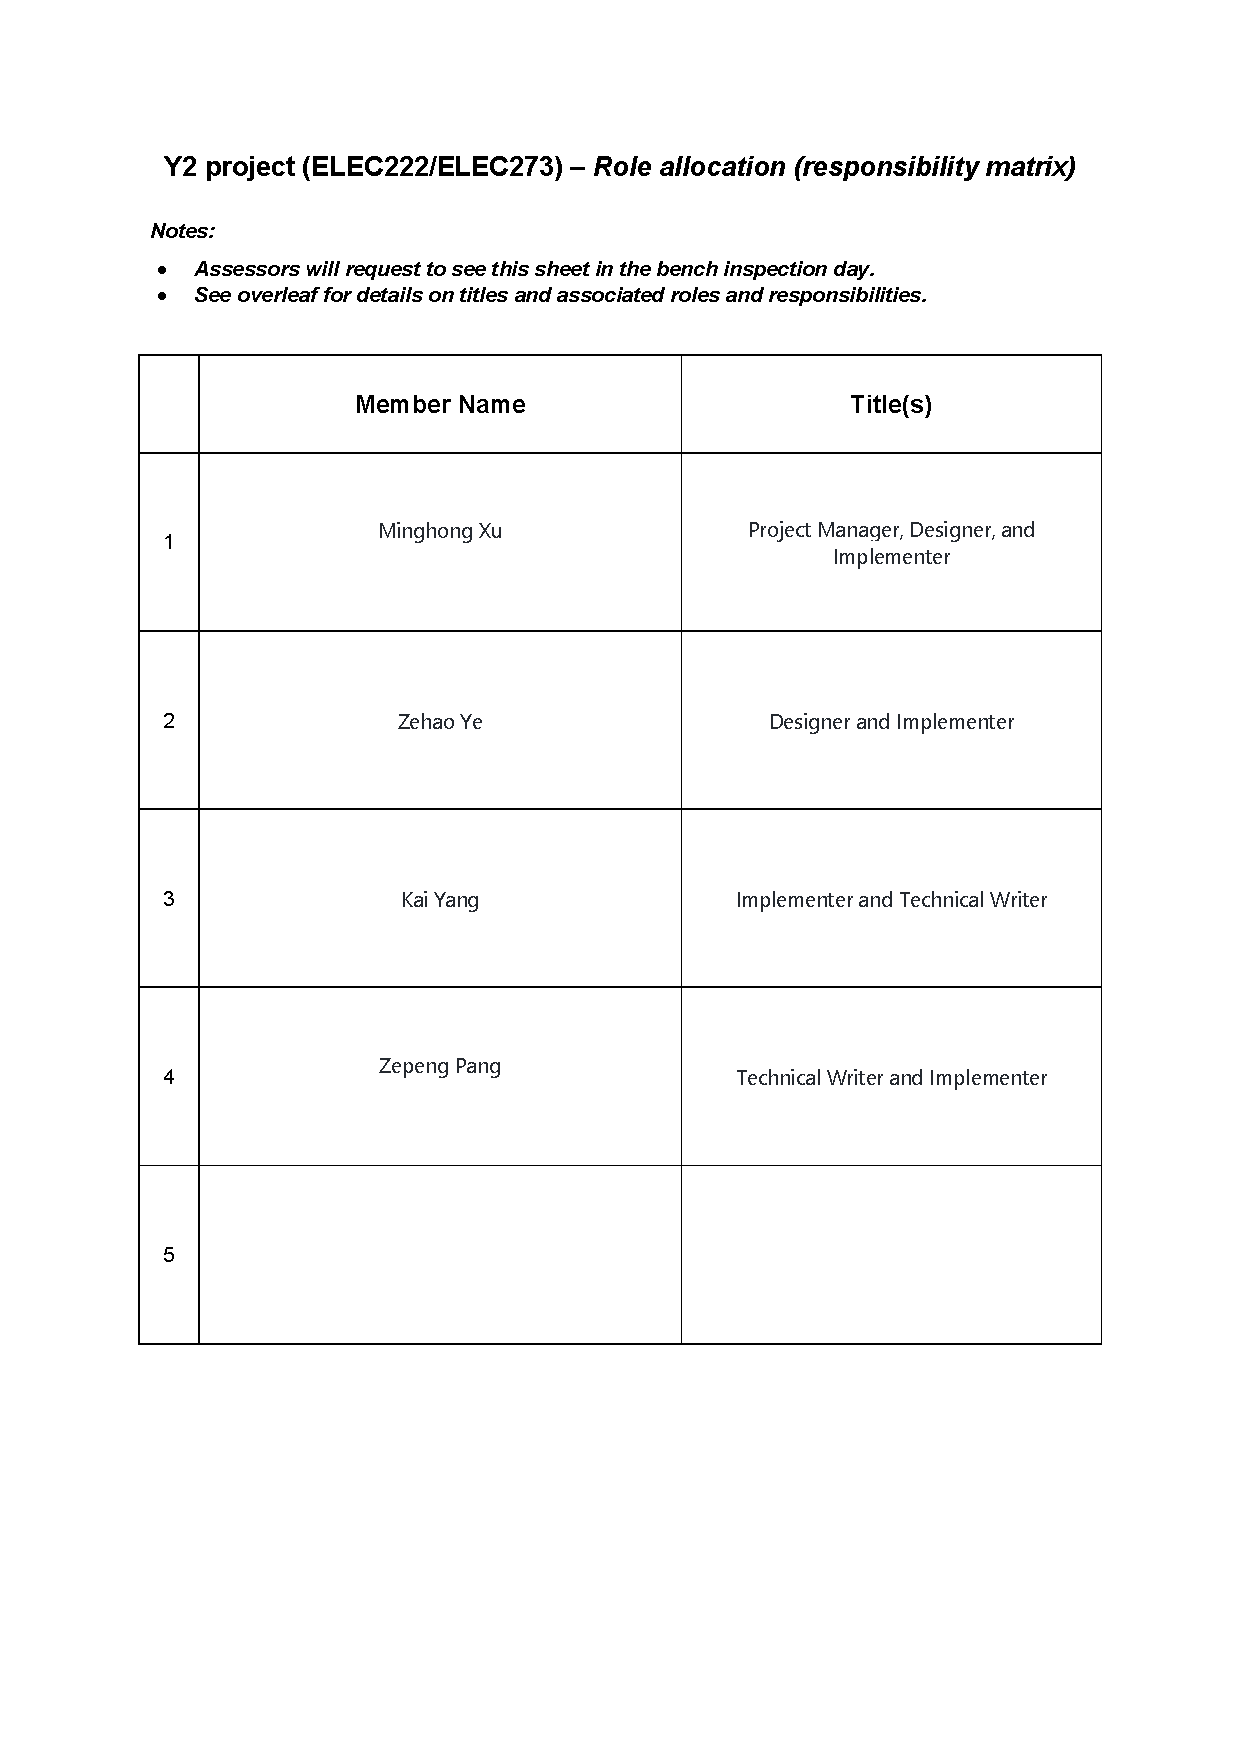
\includepdf[pages=-]{../proj_mgmt_forms/role_allocation.pdf}
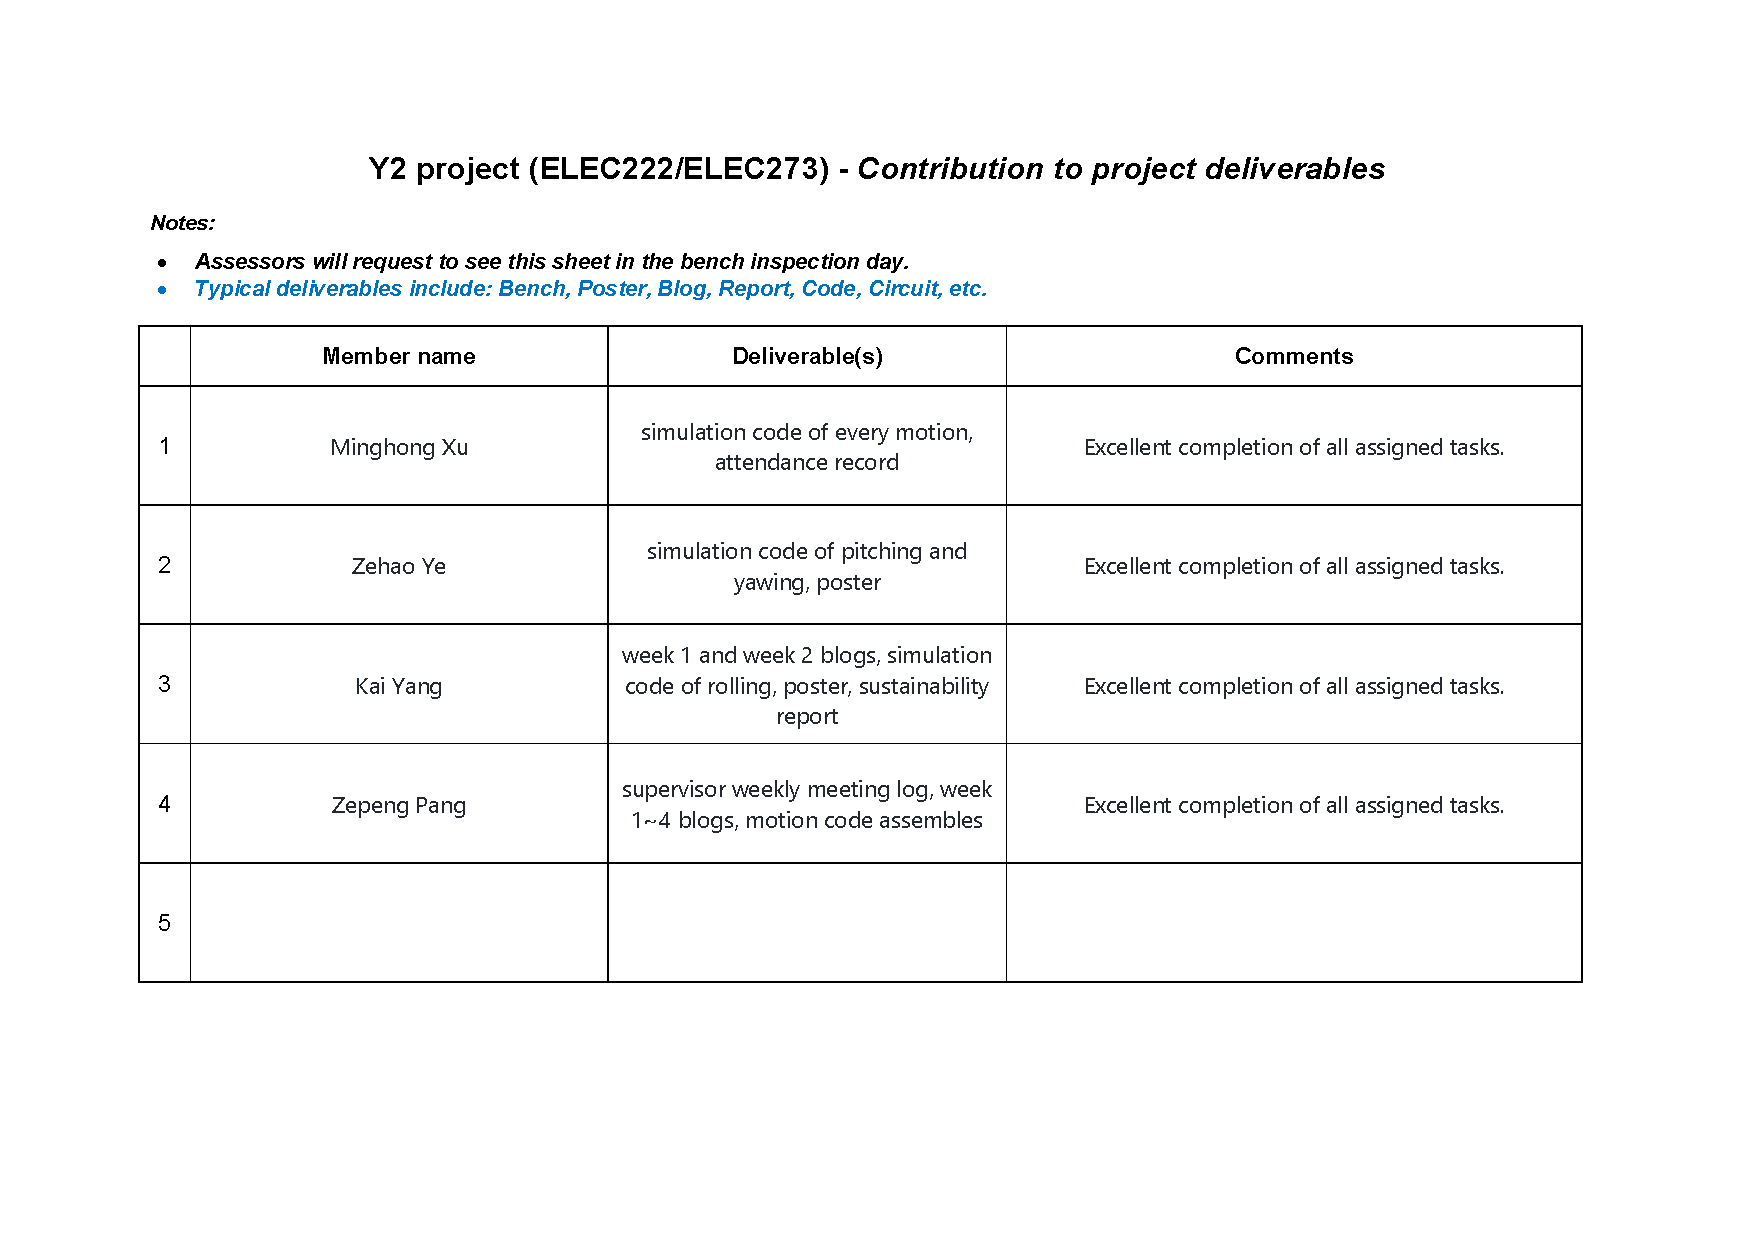
\includepdf[pages=-]{../proj_mgmt_forms/contribution_to_project_deliverables.pdf}
\includepdf[pages={2}]{../proj_mgmt_forms/advisor_meeting_log_weeks_1_2.pdf}
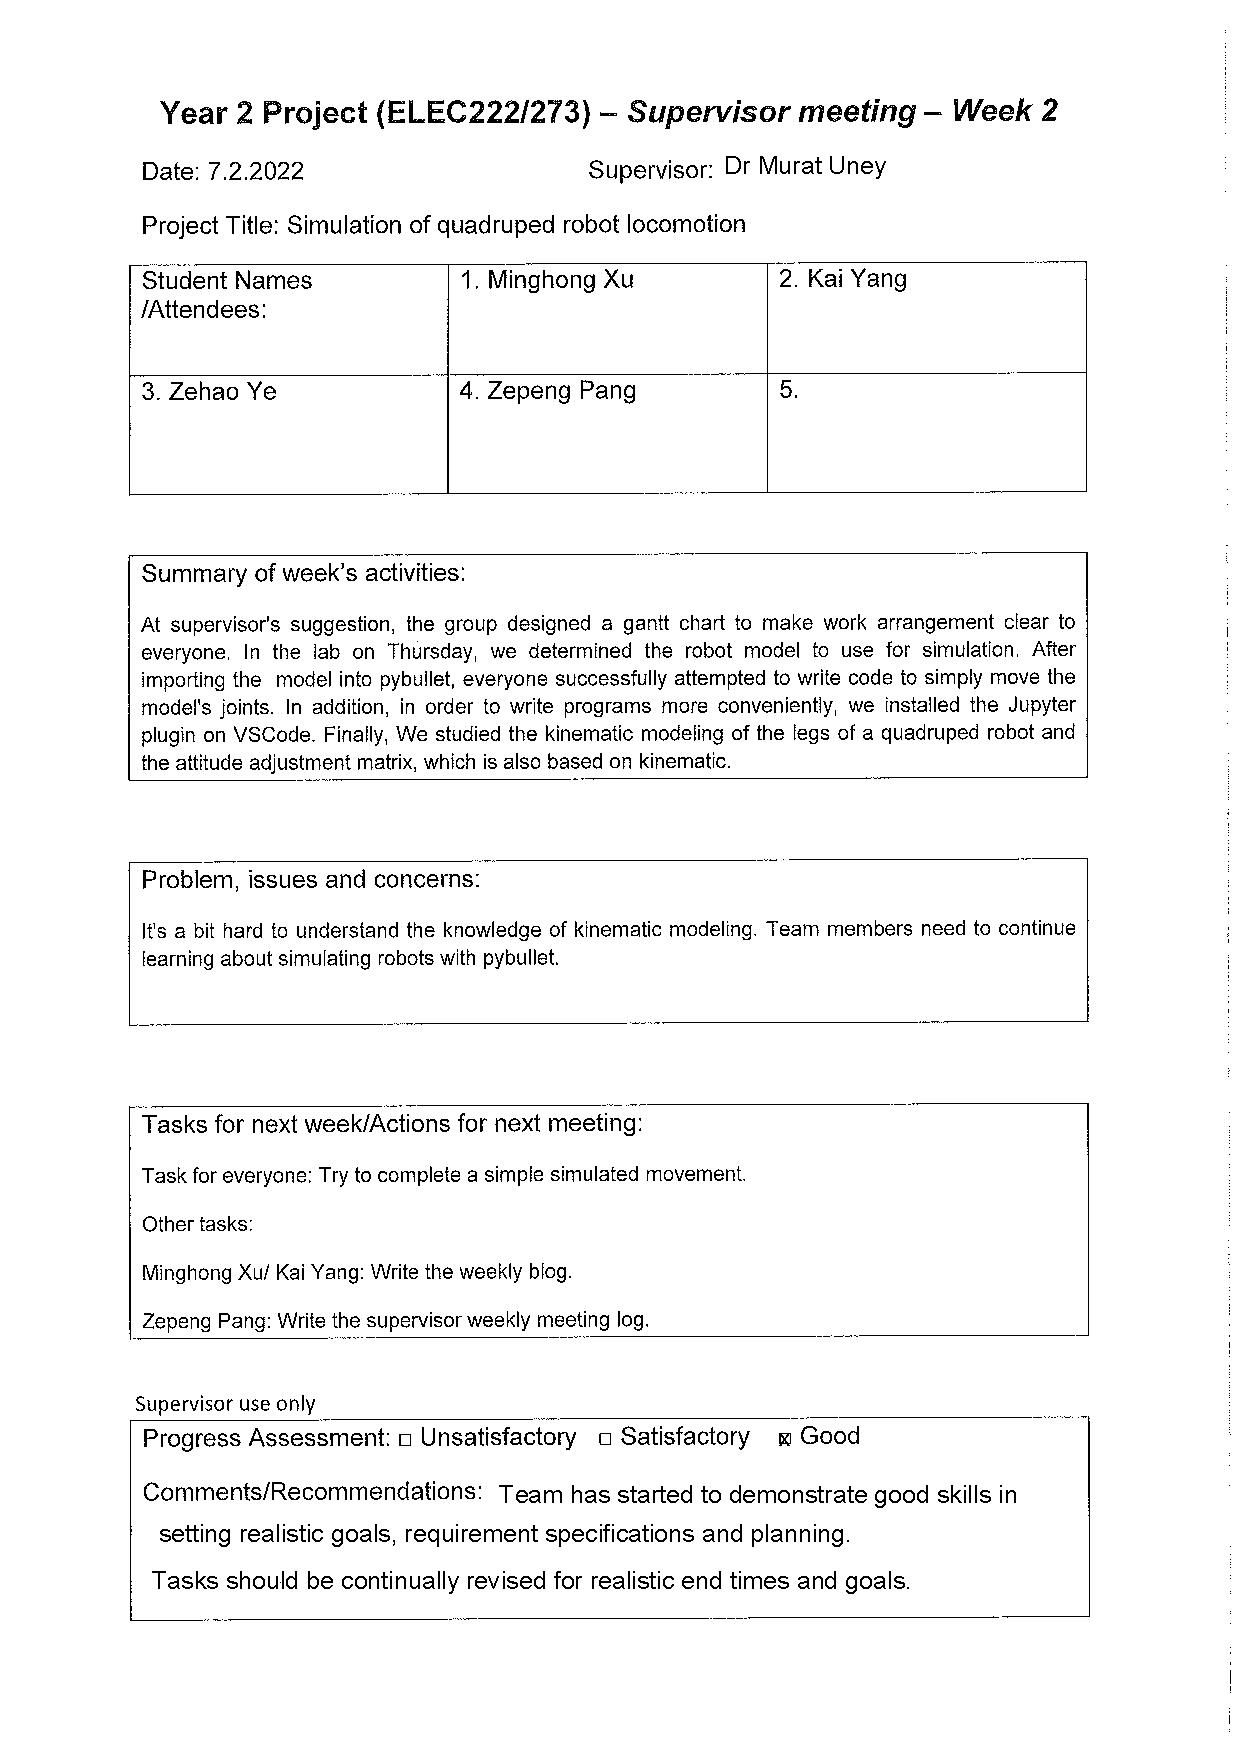
\includepdf[pages={1}]{../proj_mgmt_forms/advisor_meeting_log_weeks_1_2.pdf}
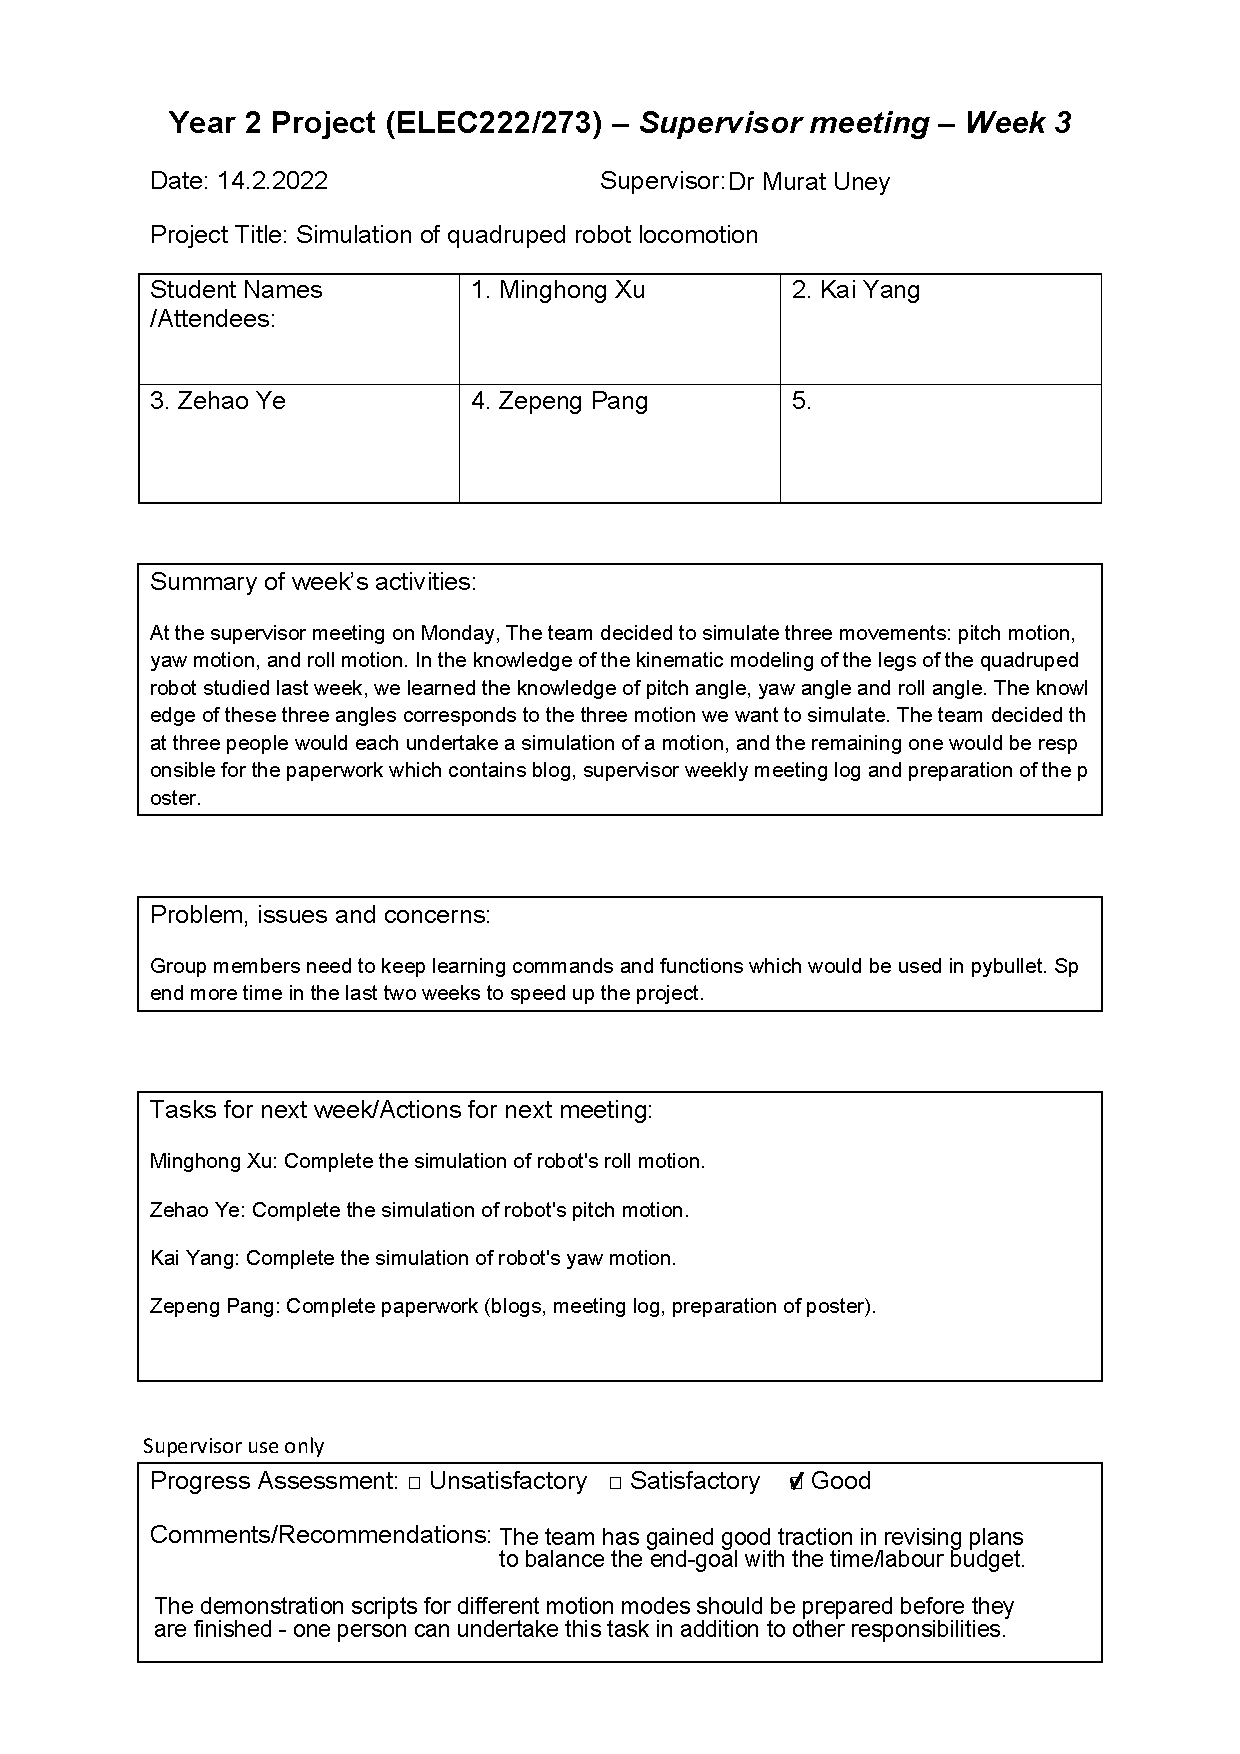
\includepdf[pages=-]{../proj_mgmt_forms/advisor_meeting_log_week_3.pdf}
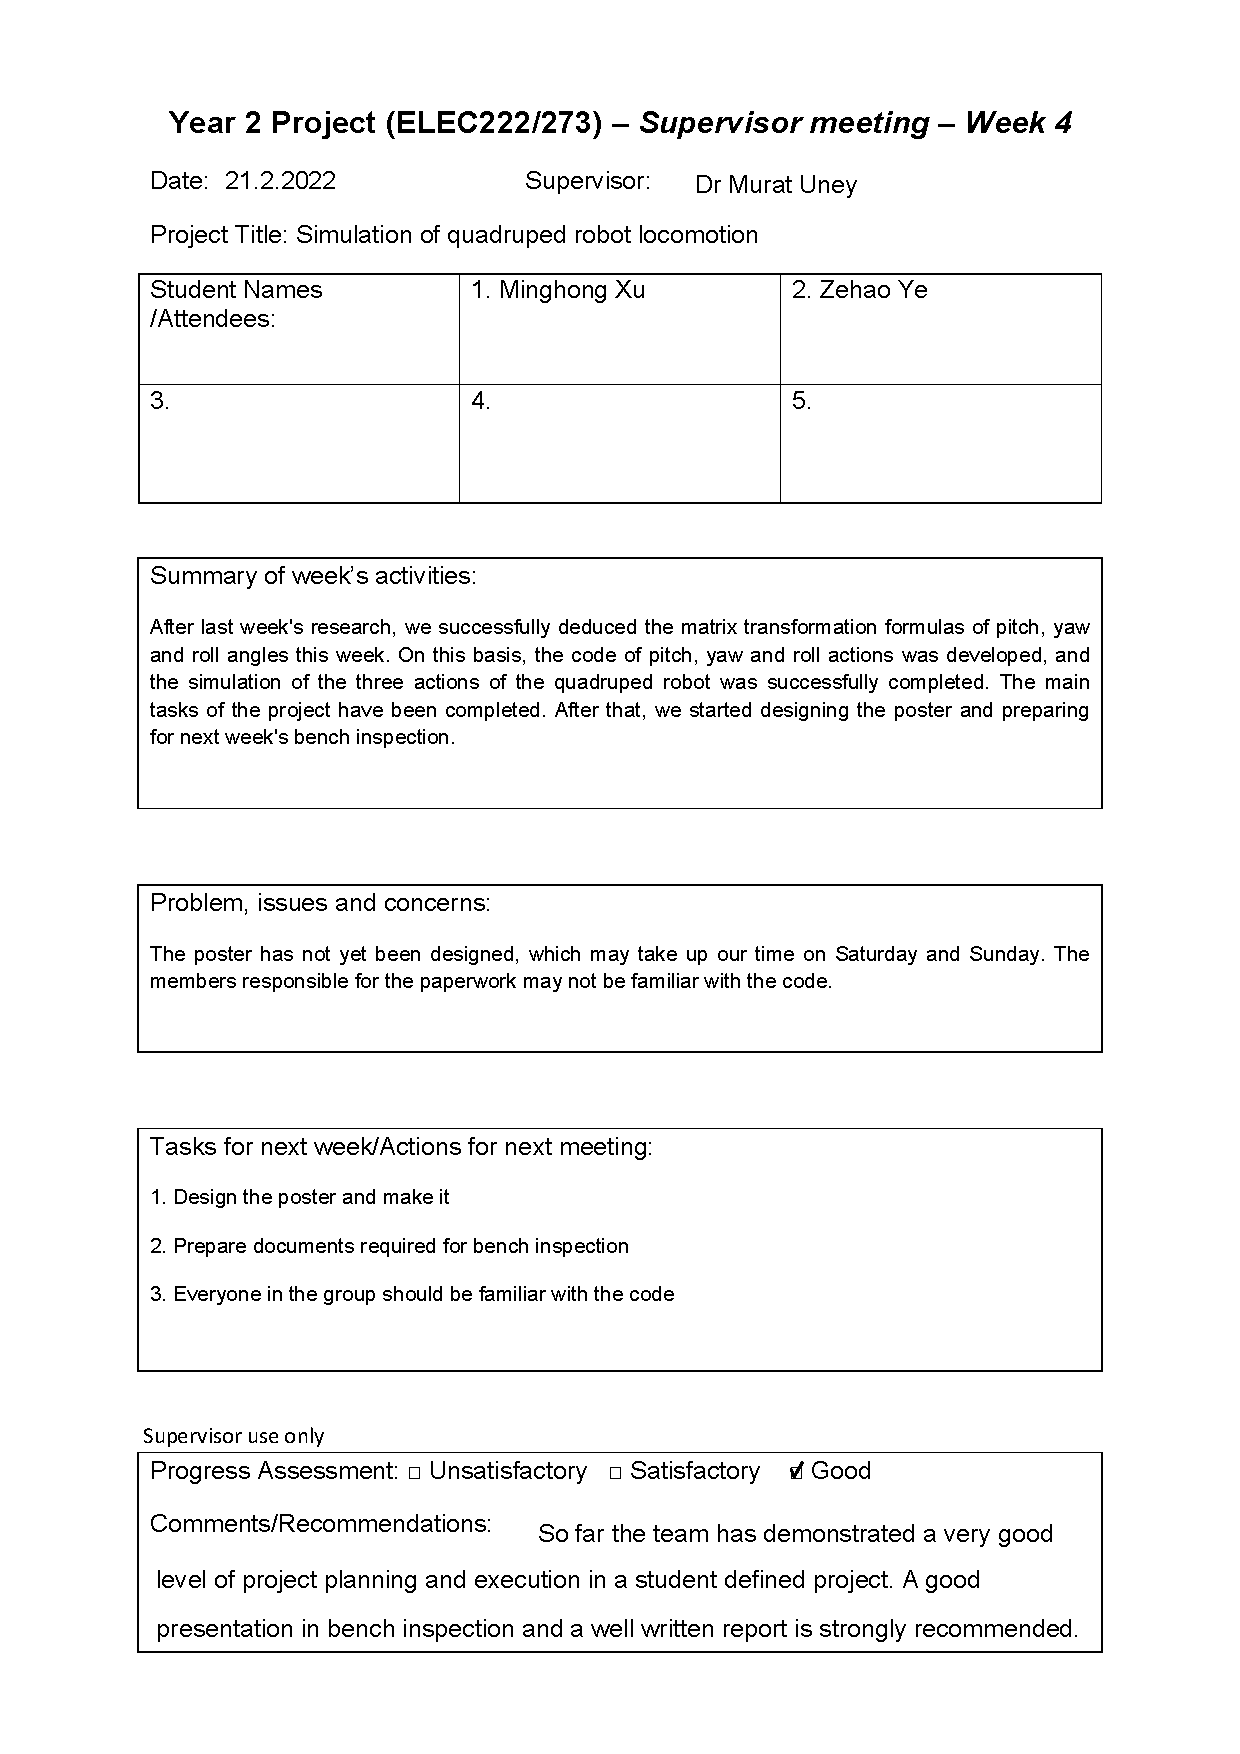
\includepdf[pages=-]{../proj_mgmt_forms/advisor_meeting_log_week_4.pdf}


\chapter{Individual contributions to the project}
\section{Minghong Xu}
\section{Zehao Ye}
In this group project, I am mainly responsible for three aspects, which are quadrupedal locomotion simulation, presentation and report. From the perspective of quadrupedal locomotion simulation, I have completed the forward and inverse kinematics derivation and matrix derivation of some parts of pitch, yaw and roll actions. The part I participated in most was pitching. Meanwhile, debug parameter section was mainly designed by me. From the perspective of presentation, I drew the poster through software. In the poster, except that the pictures of the modelling part were made by Yang Kai, other parts were completed by me. From the perspective of report, I wrote the results and analysis section. In addition, the limitations of the discussion and conclusion section are also completed by me.

\section{Zepeng Pang}

At the beginning of the project, I was responsible for the writing of the supervisor weekly meeting log and Blog. Later responsible for modifying other project management forms such as attendance record and role allocation. After the group completed the simulation of the four independent actions, I combined the four programs into a single program and added the ability to initialize the viewing angle to the program. In bench inspection, I explained the project introduction and how to model the legs of the quadruped robot. In the writing of the report, I was responsible for the writing of the title page, abstract, introduction and conclusion. In addition, I also completed the Completion of objectives of the discussion chapter and Appendix A.

\section{Kai Yang}

In this group project, I was involved in quadruped motion simulation, cartography, and report writing. Based on robotics and trigonometry, I completed the kinematic derivation and code for the roll angle part. The images used in the posters and reports of this group are all made based on professional geometric software, which can well represent the characteristics of the model. In the final report, I completed the future work outlook and intellectual property statement. In addition, I put forward a lot of ideas in the SDE report.


\chapter{Code}

\section{Library for Unitree A1 3D model}
\inputminted[fontsize=\tiny, breaklines]{python}{../simulation/liba1.py}

\section{Application for demonstration}
\inputminted[fontsize=\tiny, breaklines]{python}{../simulation/pose_control.py}
